\documentclass{article}

\usepackage{polski}
\usepackage[utf8]{inputenc}
\usepackage{graphicx}
\usepackage{float}
\usepackage{listings}
\usepackage{graphicx}
\usepackage{mathtools}
\renewcommand{\lstlistingname}{Funkcja}
\renewcommand{\theparagraph}{\alph{paragraph}) }\setcounter{secnumdepth}{4}
\lstset{language=C++,
numbers=left,
captionpos=b}

\author{Dominik Doberski, Artur Olejnik}
\title{
\huge Sprawozdanie 
\\Przetwarzanie równoległe\\
\Huge Projekt 2 PKG}

\begin{document}
\maketitle

\section{Wstęp}
\subsection{Temat}

Mnożenie macierzy - ukrycie kosztów transferu danych w czasie obliczeń (dla 5. wersji kodu), badania należy wykonać dla przetwarzania równoległego dla zbioru tablic jednocześnie dostarczanych, obliczanych i pobieranych do/z systemu PKG, porównanie z prędkością przetwarzania dla wersji 3.
\begin{itemize}
\item 5. wersja kodu -- grid wieloblokowy, obliczenia przy wykorzystaniu pamięci współdzielonej bloku wątków, zrównoleglenie obliczeń i transferu danych między pamięciami: operacyjną procesora, a globalną karty,
\item 3. wersja kodu -- grid wieloblokowy, obliczenia przy wykorzystaniu pamięci współdzielonej bloku wątków.
\end{itemize}
\subsection{Autorzy}
\begin{minipage}[t]{0.3\textwidth}
% Pierwsza kolumna (średnia)
Dominik Doberski\\
Artur Olejnik
\end{minipage}
\begin{minipage}[t]{0.15\textwidth}
% Druga kolumna (mniejsza)
132207\\
122402
\end{minipage}
\begin{minipage}[t]{0.55\textwidth}
% Trzecia kolumna (mniejsza)
dominik.doberski@student.put.poznan.pl\\
artur.olejnik@student.put.poznan.pl
\end{minipage}
\\\\\\
Grupa dziekańska I3\\
Termin zajęć: poniedziałek 16:50 
\subsection{Opis wykorzystywanej karty graficznej}
Do wykonania pomiarów wykorzystano program CodeXL. Testy zrealizowano na jednostce obliczeniowej o poniższej specyfikacji:
\begin{itemize}
\item Nazwa: Nvidia GeForce GTX 1060
\item Pamięć: 3072MB
\item Typ: dedykowana
\item CC – możliwości obliczeniowe: 6.1
\item Liczba SM: 9
\item Liczba rdzeni: 1152
\item Maksymalna liczba wątków na multiprocesor: 2048
\item Maksymalna liczba wątków na blok: 1024
\item Rozmiar osnowy: 32
\item Maksymalny rozmiar bloku: 1024x1024x64
\end{itemize}

\section{Analiza algorytmu}
\subsection{Kluczowe fragmenty kodu}
\subsubsection{Algorytm dla 3. wersji kodu}
Grid wieloblokowy, obliczenia przy wykorzystaniu pamięci współdzielonej bloku wątków:
\begin{lstlisting}[
caption={3. wersja kodu},
label=1. funkcja,
firstnumber=1]
template <int BLOCK_SIZE> __global__ void
matrixMul3(float *C, float *A, float *B, int width) {
    int bx = blockIdx.x;
    int by = blockIdx.y;
    
    int tx = threadIdx.x;
    int ty = threadIdx.y;
    
    int aBegin = width * BLOCK_SIZE * by;
    int aEnd   = aBegin + width - 1;
    int aStep  = BLOCK_SIZE;
    int bBegin = BLOCK_SIZE * bx;
    int bStep  = BLOCK_SIZE * width;
    
    float Csub = 0;

    __shared__ float As[BLOCK_SIZE][BLOCK_SIZE];
    __shared__ float Bs[BLOCK_SIZE][BLOCK_SIZE];

    for (int a = aBegin, b = bBegin; 
    	 a <= aEnd;
    	 a += aStep, b += bStep) {
        As[ty][tx] = A[a + width * ty + tx];
        Bs[ty][tx] = B[b + width * ty + tx];
        
        __syncthreads();
        
#pragma unroll
        for (int k = 0; k < BLOCK_SIZE; ++k) {
            Csub += As[ty][k] * Bs[k][tx];
        }

        __syncthreads();
    }
    
    int c = width * BLOCK_SIZE * by + BLOCK_SIZE * bx;
    C[c + width * ty + tx] = Csub;    
}
\end{lstlisting}

Funkcja ma za zadanie wyznaczenie jednej wartości macierzy $C$ przez jeden wątek. Argumentami powyższej funkcji są wskaźniki na tablice $A$, $B$ i $C$, oraz wartość $width$, która oznacza wielkość każdego wymiaru każdej macierzy.

Pierwszą czynnością, która wykonuje powyższa funkcja jest wyznaczenie numeru bloku w 3. i 4. linii kodu, następnie w 6. i 7. wyznaczane jest położenie wątku wewnątrz tego bloku. W kolejnych liniach wyznaczane są adresy macierzy $A$ i $B$ potrzebne do obliczeń. W 15. linii tworzymy zmienną lokalną $Csub$, która posłuży nam do obliczenia wartości kolejnych komórek macierzy wynikowej $C$. W linii 17. i 18. deklarowana jest pamięć współdzielona dla obu macierzy.

W pętli funkcja kopiuje wartości z obu macierzy do pamięci współdzielonej, a zaraz po tym następuje synchronizacja wątków w obrębie bloku (linie 23-26), która zapewnia nas o tym, że do pamięci współdzielonej przypisane zostały wszystkie wymagane elementy. Dyrektywa $\#pragma\ unroll$ posłuży do odwinięcia ciała pętli (linie 29-31) w szereg pojedynczych instrukcji, których zadaniem jest wyliczenie częściowego wyniku wykorzystując dane z pamięci współdzielonej. Następnie ponownie występuje bariera synchroniczna, która zapobiegnie nadpisaniu tej pamięci.

Po uzyskaniu wyniku częściowego funkcja zapisze go, już poza pętlą w 37. linii kodu, do pamięci głównej w odpowiedniej komórce macierzy $C$.

\subsubsection{Algorytm dla 5. wersji kodu}
Grid wieloblokowy, obliczenia przy wykorzystaniu pamięci współdzielonej bloku wątków, zrównoleglenie obliczeń i transferu danych między pamięciami: operacyjną procesora, a globalną karty:

\begin{lstlisting}[
caption={5. wersja kodu},
label=2. funkcja,
firstnumber=39]
template <int BLOCK_SIZE> __global__ void
matrixMulCUDA(float *C, float *A, float *B, int width) {
    int bx = blockIdx.x;
    int by = blockIdx.y;
    
    int tx = threadIdx.x;
    int ty = threadIdx.y;

    int aBegin = width * BLOCK_SIZE * by;
    int aEnd = aBegin + width - 1;
    int aStep = BLOCK_SIZE;
    int bBegin = BLOCK_SIZE * bx;
    int bStep = BLOCK_SIZE * width;

    float Csub = 0;
    
    __shared__ float As[BLOCK_SIZE][BLOCK_SIZE];
    __shared__ float Bs[BLOCK_SIZE][BLOCK_SIZE];

    __shared__ float A_shared[BLOCK_SIZE][BLOCK_SIZE];
    __shared__ float B_shared[BLOCK_SIZE][BLOCK_SIZE];

    A_shared[ty][tx] = A[aBegin + width * ty + tx];
    B_shared[ty][tx] = B[bBegin + width * ty + tx];

    for (int a = aBegin, b = bBegin; a <= aEnd; a += aStep, b += bStep) {
        As[ty][tx] = A_shared[ty][tx];
        Bs[ty][tx] = B_shared[ty][tx];

        __syncthreads();

        A_shared[ty][tx] = A[a + width * ty + tx];
        B_shared[ty][tx] = B[b + width * ty + tx];

#pragma unroll
        for (int k = 0; k < BLOCK_SIZE; ++k) {
            Csub += As[ty][k] * Bs[k][tx];
        }

        __syncthreads();
    }

    int c = width * BLOCK_SIZE * by + BLOCK_SIZE * bx;
    C[c + width * ty + tx] = Csub;
}
\end{lstlisting}

Powyższa funkcja jest zmodyfikowaną wersją poprzedniej. Jej zadaniem jest również wykorzystanie pamięci współdzielonej bloku wątków do wygenerowania częściowego wyniku macierzy $C$. Różnica polega na dodatkowej funkcjonalności, którą jest zrównoleglenie obliczeń i transfer danych pomiędzy CPU i GPU.

W linii 58. i 59. deklarujemy dodatkowe pamięci współdzielone dla macierzy $A$ i $B$, do których równolegle z obliczeniami wpisujemy dane kolejnych bloków. Przed wykonaniem każdej iteracji pętli do tych pamięci zapisywane są dane z macierzy (w 70. i 71. wierszu). Tą czynność należy wykonać również przed pierwszą iteracją (61. i 62. linia). Oznacza to, że wątki po pobraniu danych do pamięci współdzielonej nie muszą się synchronizować, ponieważ w danej iteracji nie pobierają danych wykorzystywanych od razu do obliczeń, tak jak to było w poprzednim algorytmie. W tym przypadku dane pobierane do pamięci współdzielonej z macierzy będą wykorzystywane dopiero w kolejnej iteracji, w następnym fragmencie.

\subsection{Analiza dostępu do pamięci}

\subsubsection{Dostęp do pamięci dla 3. wersji kodu}

Dostęp do danych odbywa się za pomocą pamięci współdzielonej co sprawia, że jeden wątek nie musi sam pobierać wszystkich danych z macierzy, a może do tego wykorzystać dane pobrane przez inne wątki. Takie podejście jest zdecydowanie szybsze niż wykorzystywanie tylko i wyłącznie pamięci globalnej, jednak sprawia, że wymagana jest synchronizacja po pobieraniu danych z macierzy. Wymagana jest również synchronizacja na końcu każdej iteracji, aby zapobiec podmienieniu zawartości pamięci współdzielonej, kiedy inny wątek nie zdążył wykonać jeszcze wszystkich obliczeń.

\subsubsection{Dostęp do pamięci dla 5. wersji kodu}

W tym przypadku dostęp odbywa się w trochę inny sposób. Dane z pemięci globalnej są pobierane przed iteracją, w której te dane zostaną użyte i zostają one zapisane do innego obszaru pamięci współdzielonej. Po tej operacji nie jest wymagana synchronizacja, gdyż ta pamięć nie jest wykorzystywana do obliczeń. We właściwej iteracji, która te dane potrzebuje, dane są przepisywane do nowego obszaru pamięci już bez bezpośredniego dostępu do pamięci globalnej. Ten obszar będzie już użyty do obliczeń, dokładnie tak jak w 1. funkcji, zatem synchronizacja po przepisaniu tych danych jest wymagana, tak jak ta na koniec każdej iteracji pętli zewnętrznej.

\subsection{Analiza dostępu do danych}

\subsubsection{Dostęp do danych dla 3. wersji kodu}

W celu uzyskania wyniku dla częściowego każdy wątek musi w każdej iteracji pętli zewnętrznej pobrać po 1 elemencie z macierzy $A$ i $B$. To, którym elementem macierzy $C$ zajmuje się konkretny wątek, zależne jest od położenia bloku i wątku wewnątrz tego bloku.

\begin{figure}[H]
	\centering
	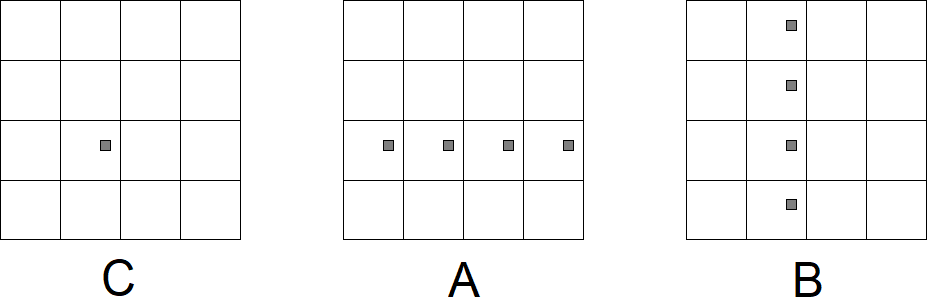
\includegraphics[width=\linewidth]{./images/3/1.png}
	\caption{Bezpośredni dostęp do danych w jednym wątku}
	\label{fig:image1}
\end{figure}

W każdej iteracji pętli zewnętrznej wątek musi pobrać dane z innego fragmentu macierzy. Wewnątrz każdego z tych fragmentów położenie pobieranego elementu jest stałe i odpowiada położeniu wątku wewnątrz bloku wątków. Powyższy rysunek przedstawia, które elementy musi pobrać wątek z macierzy $A$ i $B$ dla wyznaczenia przykładowego elementu macierzy $C$.

Oczywiście pobrane wartości nie są wykorzystywane w tej funkcji bezpośrednio. Nie jest ich też wystarczająco tyle, aby móc od razu wyznaczyć wynik cząstkowy. Należy się posłużyć elementami wyznaczonymi w pamięci współdzielonej bloku wątków. Cały blok wątków będzie w stanie odczytać elementy wszystkich fragmentów w w wierszu fragmentów macierzy $A$ i kolumnie fragmentów macierzy $B$. W każdej iteracji pamięć współdzielona przechowuje informacje o wartościach z całego jednego fragmentu dla macierzy $A$ i $B$. 

Wiemy, że do wyznaczenia jednego elementu macierzy $C$ potrzebujemy sumy iloczynów odpowiadających elementów w tym samym wierszu macierzy $A$ i kolumnie macierzy $B$, zatem otrzymane wartości po przebiegu całej pętli zewnętrznej pozwolą na wyznaczenie wartości dla całego fragmentu macierzy $C$, którym blok wątków się zajmuje.

\subsubsection{Dostęp do danych dla 5. wersji kodu}

Dla 2. funkcji dostęp do danych odbywa się w przybliżony sposób. Zmienia się miejsce, gdzie te dane są przetrzymywane w pamięci współdzielonej, oraz moment w którym te dane są pobierane (przed iteracją pętli zewnętrznej).

\section{Wyniki przeprowadzonych eksperymentów}

\subsection{Czas przetwarzania}

\begin{figure}[H]
	\centering
	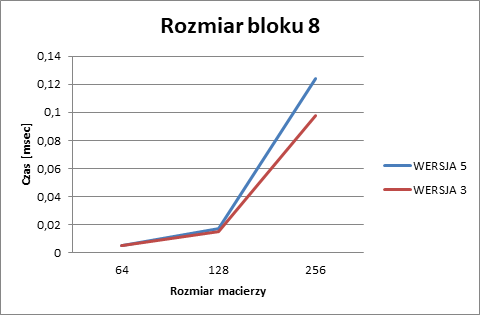
\includegraphics[width=\linewidth]{./images/graphs/time/graph1.png}
	\caption{Czas przetwarzania dla bloku o rozmiarze 8x8}
	\label{fig:grapht1}
\end{figure}

\begin{figure}[H]
	\centering
	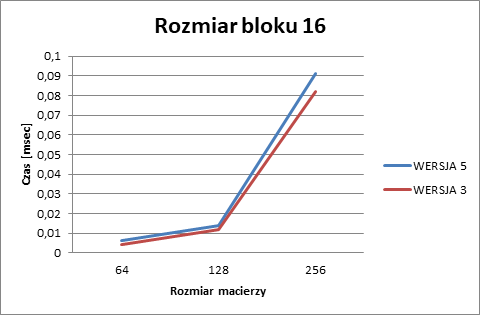
\includegraphics[width=\linewidth]{./images/graphs/time/graph2.png}
	\caption{Czas przetwarzania dla bloku o rozmiarze 16x16}
	\label{fig:grapht2}
\end{figure}

\begin{figure}[H]
	\centering
	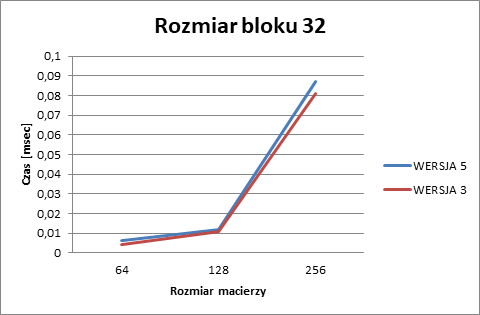
\includegraphics[width=\linewidth]{./images/graphs/time/graph3.png}
	\caption{Czas przetwarzania dla bloku o rozmiarze 32x32}
	\label{fig:grapht3}
\end{figure}

Jak widać na powyższych wykresach czas przetwarzania dla obydwu metod jest podobny. Różnice są niemal niezauważalne z niewielką przewagą dla algorytmu w wersji 3. Zwiększenie rozmiaru bolku przyspiesza przetwarzanie, jednak jest to dużo bardziej zauważalne między blokiem o rozmiarze 8 i 16, niż 16 i 32 gdzie zmiana jest nieznaczna. Zgodnie z oczekiwaniami macierz o większym rozmiarze jest liczona dłużej. Różnica między macierzą o wymiarach 64x64 i 128x128 jest niewielka, co pokazuje niepełne wykorzystanie możliwości multiprocesora przy zbyt małej instancji. Dopiero przy przetwarzaniu macierzy o rozmiarze 256x256 można zauważyć znaczące zwiększenie czasu przetwarzania.

\subsection{Prędkość przetwarzania}

\begin{figure}[H]
	\centering
	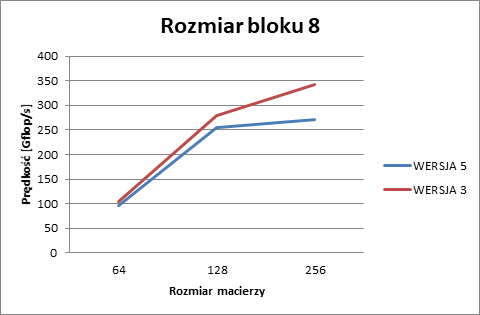
\includegraphics[width=\linewidth]{./images/graphs/fast/graph1.png}
	\caption{Czas przetwarzania dla bloku o rozmiarze 8x8}
	\label{fig:graphf1}
\end{figure}

\begin{figure}[H]
	\centering
	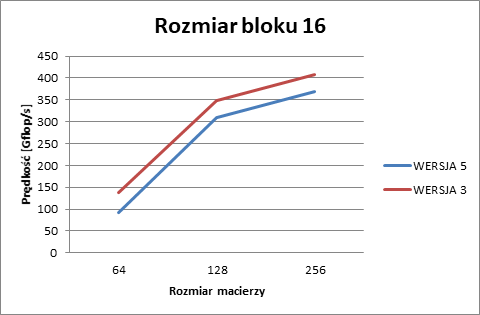
\includegraphics[width=\linewidth]{./images/graphs/fast/graph2.png}
	\caption{Czas przetwarzania dla bloku o rozmiarze 16x16}
	\label{fig:graphf2}
\end{figure}

\begin{figure}[H]
	\centering
	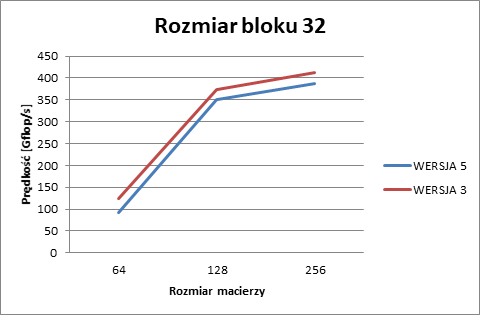
\includegraphics[width=\linewidth]{./images/graphs/fast/graph3.png}
	\caption{Czas przetwarzania dla bloku o rozmiarze 32x32}
	\label{fig:graphf3}
\end{figure}

Prędkość przetwarzania dla bloków o rozmiarach 32 i 16 jest bardzo podobna, co oznacza, że w obydwu przypadkach multiprocesor był wykorzystywany najlepiej jak można. W wersji z blokiem o rozmiarze 8, prędkość przetwarzania jest znacząco niższa, prawdopodobnie blok był zbyt mały by zająć cały multiprocesor ze względu na ogrniczenie na ilość bloków. Najniższe prędkośći przetwarzania można zaobserwować w przypadku najmniejszej instancji problemu. Dla zbyt małej ilości danych przetwarzanie na karcie graficznej działa gorzej.

\subsubsection{Stopień łączenia dostępów}

\begin{figure}[H]
	\centering
	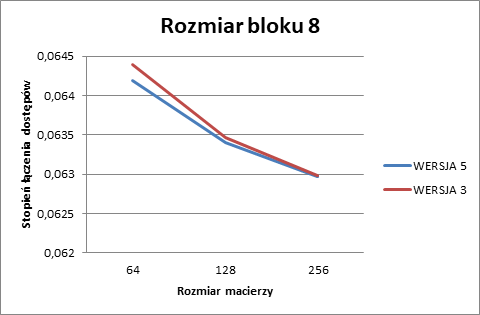
\includegraphics[width=\linewidth]{./images/graphs/dostepy/graph1.png}
	\caption{Stopień łączenia dostępów do pamięci dla bloku o rozmiarze 8x8}
	\label{fig:graphd1}
\end{figure}

\begin{figure}[H]
	\centering
	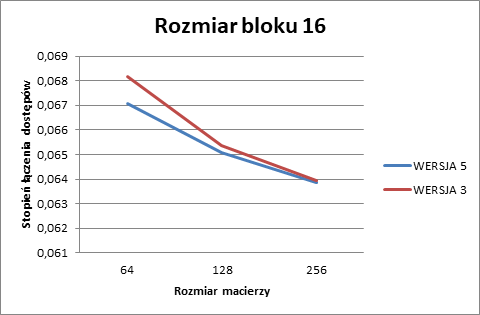
\includegraphics[width=\linewidth]{./images/graphs/dostepy/graph2.png}
	\caption{Stopień łączenia dostępów do pamięci dla bloku o rozmiarze 16x16}
	\label{fig:graphd2}
\end{figure}

\begin{figure}[H]
	\centering
	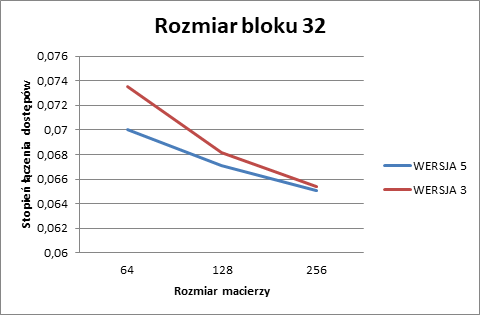
\includegraphics[width=\linewidth]{./images/graphs/dostepy/graph3.png}
	\caption{Stopień łączenia dostępów do pamięci dla bloku o rozmiarze 32x32}
	\label{fig:graphd3}
\end{figure}

\begin{figure}[H]
	\centering
	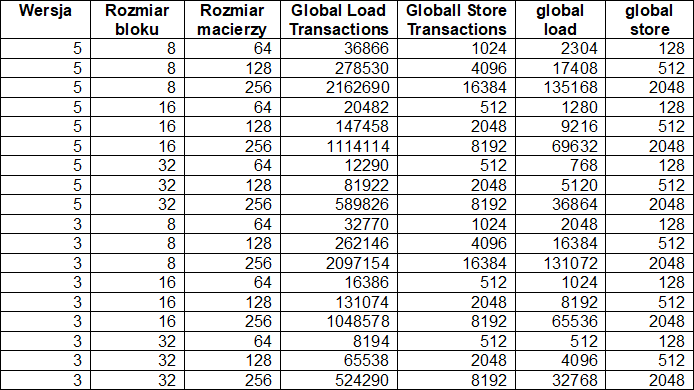
\includegraphics[width=\linewidth]{./images/tables/table1.png}
	\caption{Wyniki obliczeń stopienia łączenia dostępów do pamięci}
	\label{fig:table1}
\end{figure}

Stopień łączenia dostępów do pamięci wynosi:

\[
\frac{global\ load + global\ store}{global\ load\ transactions + global\ store\ transactions}
\]

Stopień łączenia dostępów do pamięci oznacza jak często potrzebujemy jednocześnie danych zawartych w jednej linii. Takie zapytania do pamięci można łączyć w transakcję i dzięki temu ograniczyć liczbę odwołań do wolnej pamięci. Wraz ze wzrostem rozmiaru macierzy liczba łączonych dostępów maleje. Wzrasta co prawda liczba wykonanych transakcji, jednak nieproporcjonalnie do wzrastającej liczby wszystkich odwołań. Zwiększenie rozmiaru bloku nieznacznie poprawia sytuację, ze względu na miejszą liczbę wątków.

\subsection{Zajętość multiprocesora}

\begin{figure}[H]
	\centering
	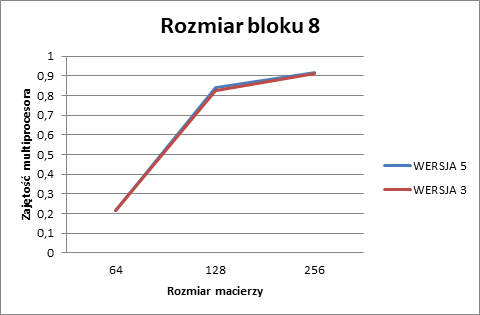
\includegraphics[width=\linewidth]{./images/graphs/zajetosc/graph1.png}
	\caption{Zajętość multiprocesora dla bloku o rozmiarze 8x8}
	\label{fig:graphz1}
\end{figure}

\begin{figure}[H]
	\centering
	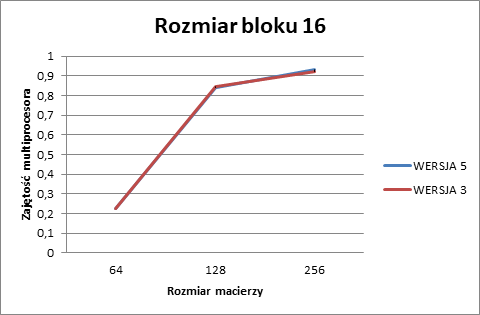
\includegraphics[width=\linewidth]{./images/graphs/zajetosc/graph2.png}
	\caption{Zajętość multiprocesora dla bloku o rozmiarze 16x16}
	\label{fig:graphz2}
\end{figure}

\begin{figure}[H]
	\centering
	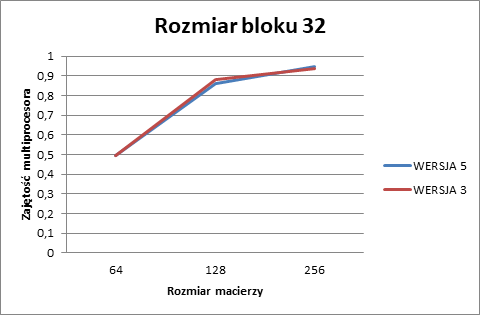
\includegraphics[width=\linewidth]{./images/graphs/zajetosc/graph3.png}
	\caption{Zajętość multiprocesora dla bloku o rozmiarze 32x32}
	\label{fig:graphz3}
\end{figure}

\begin{figure}[H]
	\centering
	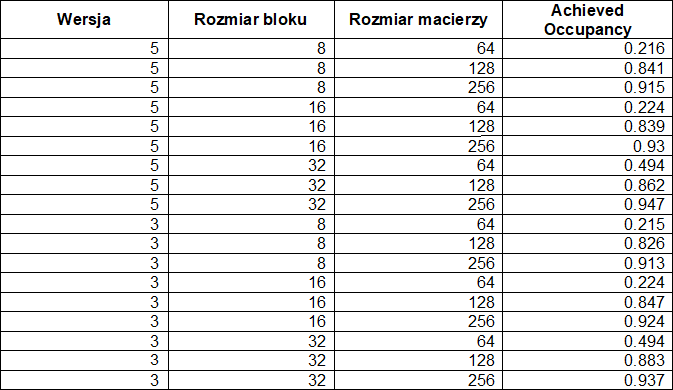
\includegraphics[width=\linewidth]{./images/tables/table2.png}
	\caption{Wyniki odczytu zajętości multiprocesora}
	\label{fig:table2}
\end{figure}

Zajętość multiprocesora odczytujemy z wartości Achieved Occupancy z programu Nvidia visual profiler. Oznacza ona stosunek aktywnych wiązek do maksymalnej liczby wiązek w SM. Jak widać na powyższych wykresach zgodnie z przewidywaniami dla macierzy o rozmiarze 64x64 mamy zbyt mało wiązek by móc w pełni wykorzystać możliwości multiprocesora. Dopiero rozmiar 128x128 i 256x256 daje wartości bliskie 1, czyli maksymalnej możliwej zajętości. Zwiększenie rozmiaru bloku również nieznacznie poprawia tę wartość.

\subsection{Współczynnik poziomu rozbieżności przetwarzania}

\begin{figure}[H]
	\centering
	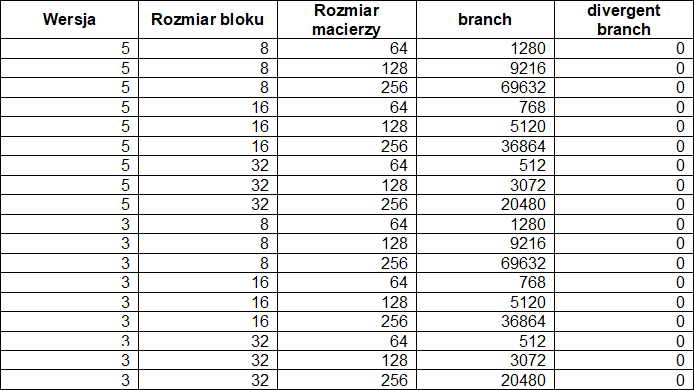
\includegraphics[width=\linewidth]{./images/tables/table3.png}
	\caption{Wyniki odczytu współczynnika rozbieżności przetwarzania}
	\label{fig:table3}
\end{figure}

Współczynnik poziomu rozbieżności przetwarzania wynosi:

\[
\frac{branch - divergent\ branch}{branch}
\]

Współczynnik poziomu rozbieżności przetwarzania wiązek w kodzie to liczba gałęzi rozbierznych które powstają w kodzie przy instrukcjach warunkowych. Wówczas wiązka musi przetwarzać różne wersje kodu co bardzo źle wpływa na efektywność przetwarzania. Jeżeli wszystkie wątki wybiorą tę samą wersję rozwiazania instrukcji warunkowej, to nie będzie gałęzi rozbierznych. Obie wersje kodu które testujemy nie posiadają instrukcji warunkowych, dlatego zgodnie z oczekiwaniami wartość ta, jest zawsze równa 1.

\section{Wnioski końcowe}
Zrównoleglenie obliczeń nie wpłynęło w pozytywnie na działanie algorytmu.

\end{document}